\chapter{Présentation des accidents graves dans les réacteurs à eau pressurisée}
\section{Fonctionnement d'un réacteur à eau pressurisée}

En France 56 réacteurs nucléaires dispersés sur 18 sites sont actuellement en service, ce parc est uniquement composé de réacteur à eau pressurisée (REP). Ces réacteurs représentent 70\% de la production électrique dans l'hexagone en 2019 d'après RTE, la France étant le deuxième plus gros producteur d'énergie nucléaire dans le monde après les États-Unis. Les puissances fournies par ces réacteurs dit de deuxième génération varient entre 900 MWe et 1450 MWe. Un réacteur de troisième génération d'une puissance de 1650 MWe (EPR - European pressurized reactor) est actuellement en construction sur le site de Flamanville, ce type de réacteur prend en compte le retour d'expérience des réacteurs actuels intégrant notamment plus d'éléments de sûreté. La construction de 6 nouveaux EPR a été annoncée et 8 autres pourraient voir le jour. \\

\begin{figure}[h!]
	\centering
	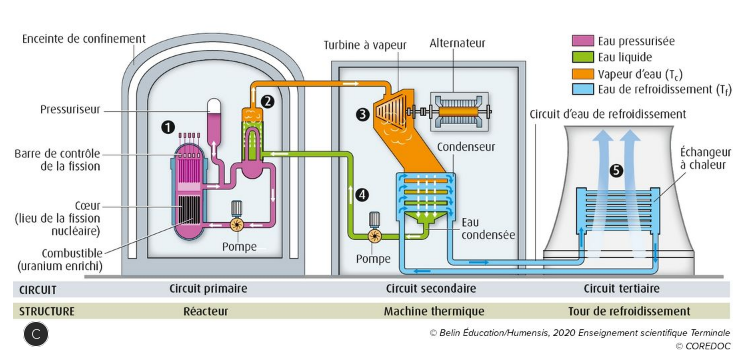
\includegraphics[width=0.8\linewidth]{figure/sch_centrale1}
	\caption[Schéma de principe d'une centrale nucléaire de type REP]{Schéma de principe d'une centrale nucléaire de type REP, (d'après manuelnumeriquemax.belin.education)}
	\label{fig:schcentrale1}
\end{figure} 
Les REP sont des réacteurs de la famille des réacteurs à eau légère, de l'eau est utilisée comme fluide caloporteur et modérateur, de plus cette eau est pressurisée à 155 bars pour éviter un changement d'état liquide-gaz dans le circuit primaire et ainsi obtenir un meilleur coefficient d'échange thermique, à l'entrée de la cuve la température de l'eau est 290\textdegree C et la température de sortie de cuve en fonctionnement nominal est de 330\textdegree C.

Le c\oe ur du réacteur est composé d'assemblages combustibles comportant chacun 264 crayons combustibles, 24 tubes pouvant contenir les crayons d'une grappe de commande ainsi qu'un tube servant à l'instrumentation. La gaine est constituée de Zircaloy qui est un alliage composé principalement de zirconium ($Zr$), les pastilles ont un diamètre de 8.2mm et sont empilées dans une gaine d'épaisseur 0.6mm et d'une longueur d'environ 4m (dépendante du palier du réacteur). Le zirconium est utilisé pour sa bonne résistance à la corrosion et sa faible absorption neutronique. Chaque c\oe ur est composé d'un ensemble d'assemblage combustible (241 pour l'EPR, embarquant au total 144.2 tonnes d'uranium enrichi) qui doivent être renouvelés périodiquement tous les 12 à 18 mois par quart ou tiers de c\oe ur.

\begin{figure}[H]
	     \begin{subfigure}[t]{0.45\textwidth}
	     	\centering
	         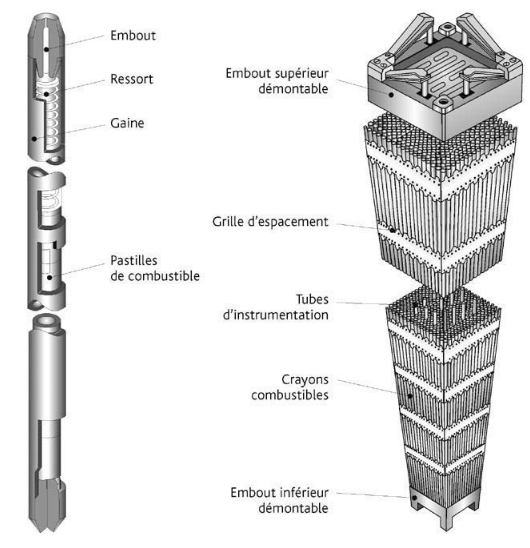
\includegraphics[width=1\textwidth]{figure/assemb.png}
	         \caption{Schéma d'un crayon combustible et d'un assemblage combustible}
	         \label{subfig:example-image-c}
	     \end{subfigure}%
     	\hfil
     	\begin{subfigure}[t]{0.45\textwidth}
     	\centering
     	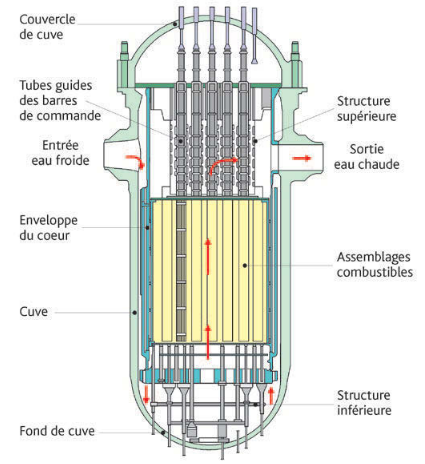
\includegraphics[width=0.99\textwidth]{figure/coeur_complet.png}
     	\caption{Schéma d'ensemble de d'une cuve d'un REP}
     	\label{subfig:example-image-c}
    	 \end{subfigure}
	     \caption{Schéma des constituants d'un c\oe ur de réacteur de type REP d'après \cite{ clement_les_2020} }
	     \label{fig:test_subfigure}
	\end{figure}
\section{Sûreté et accidents graves pour les REP}
Les questions de sûreté sont intrinsèquement liées à l'exploitation d'une centrale nucléaire tant les conséquences d'un potentiel accident peuvent être importantes. Ainsi dès le début des années 1970 le concept de défense en profondeur a été mis en place, ce concept se matérialise par la mise en place de lignes de défense successive indépendante. Pour les REP on compte 3 barrières de confinement de la radioactivité :
% \\
%\begin{minipage}[c]{0.3\linewidth}
%	\begin{enumerate}
%		\item La gaine combustible
%		\item La cuve
%		\item Le bâtiment réacteur
%	\end{enumerate}
%\end{minipage} \hfill
%\begin{minipage}[c]{0.65\linewidth}
%	\centering
%	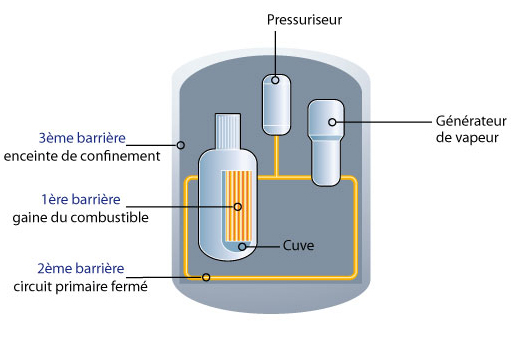
\includegraphics[width=0.7\linewidth]{figure/irsn_barriere-confinement.png}
%	\captionof{figure}{Schéma des barrières de confinement (d'après irsn.fr)}
%\end{minipage}
%\vspace{0.5cm}

\begin{enumerate}
	\item La gaine combustible
	\item La cuve
	\item Le bâtiment réacteur
\end{enumerate}
De plus les variations par rapport au régime nominal sont classés selon l'échelle INES (International Nuclear Scale Event), cette échelle permet de classifier les accidents et leurs gravités, elle comporte huit échelons allant d'un simple écart (plusieurs centaines de cas par an en France) à l'accident majeur. Les accidents correspondent aux paliers 4 à 7 et se différencient de l'incident du fait de la perte d'intégrité de la première barrière résultante de la fusion du c\oe ur, le produit de cette fusion est alors appelé corium.
\begin{figure}[h!]
	\centering
	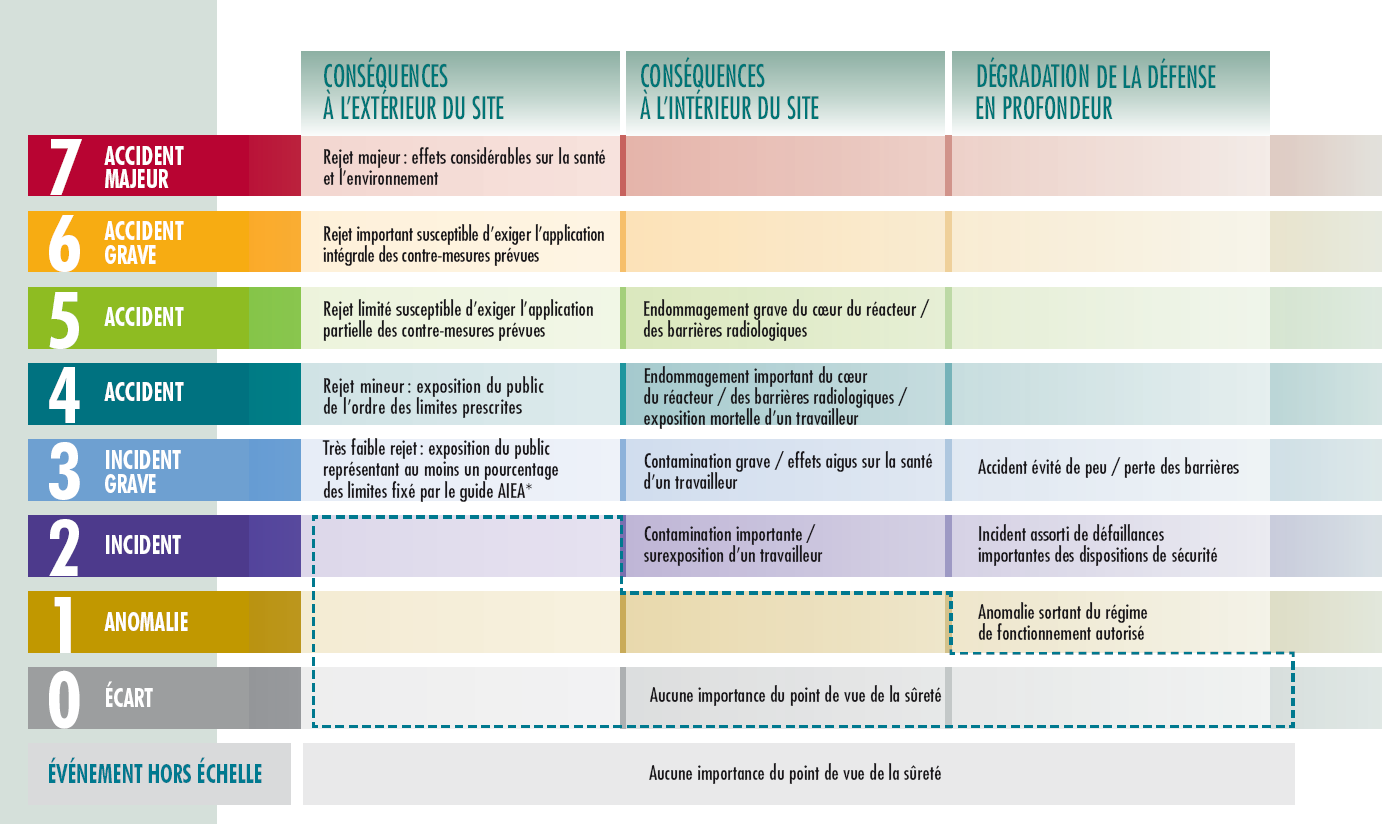
\includegraphics[width=0.7\linewidth]{figure/echelle-ines-article}
	\caption[Echelle de classification des écarts aux régimes nominal INES]{Echelle de classification des écarts aux régimes nominal INES (d'après ASN)}
	\label{fig:echelle-ines-article}
\end{figure}\\
Les accidents possibles dans les REP sont séparés en deux grandes catégories, les accidents de réactivité et les Accidents de Perte de Réfrigérant Primaire (APRP). Les accidents de réactivité sont dû à une accélération brutale de la réaction en chaîne entraînant une augmentation de puissance thermique produite. Les Accidents de Perte de Réfrigérant Primaire (APRP) résultent quant à eux d'une fuite dans le circuit primaire ou un arrêt de la circulation du fluide caloporteur. Dans la suite nous traiterons uniquement de cette seconde famille d'accident.
D'après \cite{kolev_multiphase_2015} voici le scénario de fonte du c\oe ur :
\begin{itemize}
	\item[$\bullet$] \underline{Entre 800 et 900 \textdegree C :} L'augmentation de la pression à l'intérieur de la gaine en zirconium provoque un gonflement puis une rupture de cette dernière.
	\item[$\bullet$] \underline{Entre 900 et 1300 \textdegree C :} Début de la réaction fortement exothermique d'oxydation de la gaine. A cet instant une forte proportion de la puissance thermique dégagée provient de cette réaction. La molécule d'eau est dissociée, l'oxygène est absorbé par la surface métallique et l'hydrogène est libéré. L'absorption de l'hydrogène dans les fissures du métal le fragilise davantage et accélère le processus de défaillance de la gaine. De plus l'apparition de fissure augmente la surface de réaction provoquant une accélération de la réaction.
	\item[$\bullet$] \underline{Entre 1300 et 1400 \textdegree C :} Apparition d'alliages constitués des matériaux composant la gaine (principalement Zr) et de l'acier présent dans la cuve.
	\item[$\bullet$] \underline{Entre 1400 et 1500 \textdegree C :} Fusion et rupture des structures métallique du c\oe ur. Libération des composant en phase gazeuse du combustible.
	\item[$\bullet$] \underline{Entre 1500 et 1850 \textdegree C :} Point de fusion du zirconium, dissolution du dioxyde d'uranium UO$_2$ par le zirconium en fusion, apparition de l'alliage (U,O,Zr)
	\item[$\bullet$] \underline{Entre 2000 et 2650 \textdegree C :} Fusion du ZrO$_2$, dissolution de l'UO$_2$ dans le ZrO$_2$ fondu et formation de la solution liquide UO$_2$-ZrO$_2$.
\end{itemize}
Une fois le c\oe ur fondu celui-ci se relocalise dans le fond de la cuve réacteur et il devient nécessaire d'adopter une stratégie pour refroidir ce bain.

\section{Stratégie de rétention du corium en fond de cuve (IVR)}
Une fois le c\oe ur fondu celui-ci se relocalise au fond de la cuve du réacteur. Pour limiter les conséquences d'un accident une stratégie vise à maintenir ce corium dans le fond de cette cuve, c'est la stratégie d'In-Vessel Retention (IVR). Pour cela on cherche à refroidir la cuve par l'extérieur. Cette stratégie est étudiée depuis les années 90 et mise en \oe uvre sur des réacteurs de faible puissance. \\
Le comportement du corium en fond de cuve est alors régi par deux principaux phénomènes :
La thermohydraulique du bain, avec un écoulement turbulent soumis à des rouleaux de convection (instabilité de Rayleigh-Bénard) dans la phase oxyde, d'autre part la thermochimie régit quant à elle le comportement des phases et leurs équilibres. \\
Les premières études du comportement du bain de corium ont été réalisés pour des bains stationnaires. Il a été montré qu'en régime stationnaire le bain est stratifié avec une phase oxyde et une phase métal, cependant en fonction de l'accident la couche de métal peut être lourde (i.e plus que l'oxyde et donc être en dessous) ou légère. Les différents cas sont obtenus via des différences de conditions initiales (fraction massique d'acier, degré d'oxydation du zirconium, le rapport molaire entre l'uranium et le zirconium dans la phase oxyde et la température du bain). Des études plus récentes ont montré que le transitoire reste plus contraignant et fait donc l'objet d'étude plus poussée. Lors du transitoire des phénomènes d'inversion de phase sont observés, une partie du métal de la phase légère s'alourdit sous l'effet d'un transfert de masse et des gouttes tombent, puis sous l'effet d'un même transfert de masse la phase lourde remonte. On observe alors trois couches : une couche d'oxyde, une de métal léger localiser au dessus de la couche d'oxyde et une couche de métal lourd en fond de cuve ainsi qu'une croûte située entre les phases liquides et la cuve est également présente. Finalement on se retrouve dans la situation suivante :
\begin{figure}[h!]
	\centering
	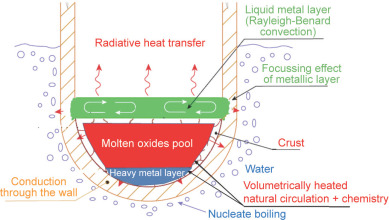
\includegraphics[width=0.6\linewidth]{figure/IVR_schema}
	\caption[Schéma du comportement du corium en fond de cuve]{Schéma du comportement du corium en fond de cuve, d'après pourlascience.fr}
	\label{fig:ivrschema}
\end{figure}\\

 

La couche de métal lourd se forme à partir d'un transfert de masse entre la phase oxyde et métal léger créant des gouttes d'acier lourd se relocalisant en fond de cuve. L'essai expérimental MASCA RCW, au cours duquel 45kg de corium ont été mis en contact avec 4kg d'acier de telle sorte que l'ensemble soit sous équilibre thermochimique dans un état de stratification comportant une phase lourde,a permis d'observer les gouttes lors de la descente, cependant la remontée de la phase lourde vers la phase légère n'a jamais été observée, l'essai ayant été arrêté au bout de 20 minutes le régime stationnaire n'a pas été atteint (voir figure \ref{fig:masca}).
 \begin{figure}[H]
	\centering
	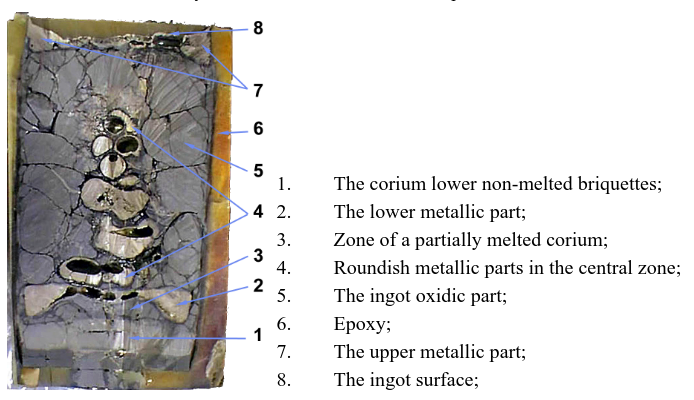
\includegraphics[width=0.7\linewidth]{figure/masca}
	\caption[Résultat MASCA-RCW 100]{Résultat MASCA-RCW 100 ,d'après \cite{}}
	\label{fig:masca}
\end{figure}


